\documentclass[doc, a4paper, apacite]{apa6}

\usepackage[american]{babel}

\usepackage{csquotes}
%\usepackage[style=apa,sortcites=true,sorting=nyt,backend=biber]{biblatex}
%\DeclareLanguageMapping{american}{american-apa}
\usepackage{threeparttable}
\usepackage{booktabs} % For nice tables
\usepackage{amsmath} % For \text{} function 
\usepackage{setspace}

\title{Looking at bumping up uncertainty and effects of background.}
\shorttitle{DSTL08}

\author{Charlotte E. R. Edmunds, Adam Harris, Magda Osman}
\affiliation{Queen Mary, UCL, University of London \\ 26 November 2020}

%\leftheader{Edmunds}

%\abstract{}
%
%\keywords{}

\begin{document}
\maketitle
\doublespacing

\section{Method}
\subsection{Participants}
Based on the previous experiment, we recruited 480 participants through Prolific Academic, 80 participants per condition. 
Due to the particulars of the task, we did not not recruit participants that are colour blind. 
Participants were paid \pounds1.25 for their participation. 

Exclusions will aim to remove those participants that are either bots or failed to concentrate. 
Participants will also be excluded if they fail to reach the criterion on the categorisation training task. 
If participants fail to successfully learn the categorisation task, they will not continue to the monitoring task and will not be paid for their time. 
This fact will be made explicit in the advert on Prolific Academic and in the consent form. 

\subsection{Materials}
This experiment was run online using JavaScript. 

\subsection{Design}
The experiment will have a 3 (Uncertainty presentation: Control, Categorical, Uncertainty) by 2 (Background: Black, Radar) between-subjects design. 
Participants will view one of the uncertainty presentation condition displayed on one of two background: either black as in Experiments DSTL02 and DSTL03 or black with a green radar-esque rings (as shown in Figure~\ref{fig:radar}). 

\begin{figure}
	\centering
	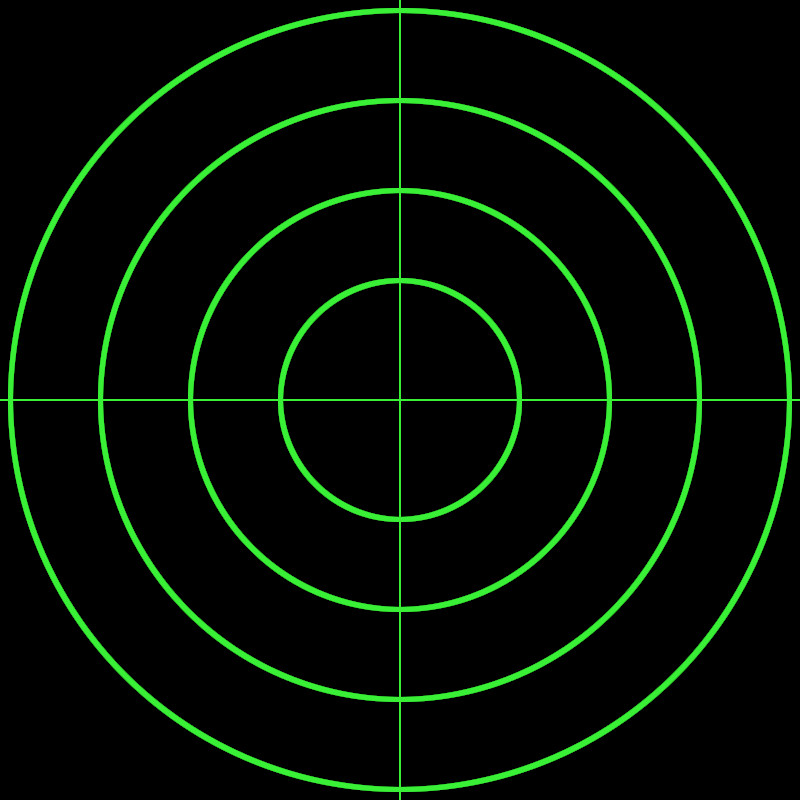
\includegraphics[width=0.5\textwidth]{images/radar.jpg}
	\caption{}
	\label{fig:radar}
\end{figure}

There are three types of uncertainty presentation:
\begin{enumerate}
	\item In the control condition, there will be four categories of entities: Unknown, Friendly, Hostile and Neutral.\\
	\item In the categorical condition, there will be six categories of entities: Unknown, Friendly, Assumed Friendly, Hostile, Assumed Hostile and Neutral. The Assumed- and Certain- versions of a categorisation (e.g. Friendly) will be different colours. 
	\item In the uncertainty condition, there will be six categories of entities: Unknown, Friendly, Assumed Friendly, Hostile, Assumed Hostile and Neutral. In this condition, the Assumed- and Certain- versions of a categorisation (e.g. Friendly) will be the same colour, where the Certain- version is a filled circle and the Assumed- version is unfilled. 
\end{enumerate}

\subsection{Stimuli}
The stimuli will be circles $30px$ in diameter. 
To mimic the displays found on Naval vessels, each circle will have a randomly generated six-digit alphanumeric code that floats next to it. 
Figure~\ref{fig:conditionColours} shows the colour mappings for the control conditions in the previous experiment and both colour way conditions in the current experiment. 

The entities will be circles that are either grey or one of five colours. 
The grey circle will have a brightness of 60\%, rgb(153, 153, 153). 
The colours will all be of equal saturation (60) and brightness (90). 
They will be presented in six colours: red (H360, rgb(230, 92, 92)), yellow (H72, rgb(202, 230, 92)), green (H144, rgb(92, 230, 147)), blue (H216, rgb(92, 147, 230)), and purple (H288, rgb(202, 92, 229)).
Across all conditions, Hostile will be red, and Unknown will be yellow. 
In the Blue conditions, Friendly will be blue and Neutral green. 
In the Green conditions, Friendly will be green and Neutral blue. 
In the categorical condition, Assumed Friendly and Assumed Hostile will be randomly assigned to grey and purple. 
In the uncertainty condition, Assumed Friendly and Assumed Hostile will be an unfilled circle the same colour as Friendly and Hostile entities respectively. 

\subsection{Procedure}

The experiment presents coloured circles moving on a black background, $800px$ square. 
The experiment has two phases: categorisation training and the monitoring task.
The categorisation training phase remains unchanged from DSTL02.  

\subsubsection{Categorisation training}
In this section, participants will learn which colour is associated with which label. 
The instructions for this task are displayed below. 
On each trial, a single stimulus will be shown, on a black background. 
The order of the stimuli shown will be pseudo-randomised: for each block of four or six stimuli (depending on the condition) participants will see all the possible stimuli in a random order. 
Along the top of the screen, buttons will be displayed showing the available options (either four or six depending on the condition). 
To respond participants click on the appropriate options and then receive feedback for one second. 
If they respond correctly, the feedback reads ``Correct'' in white plus a reinstatement of the correct answer in white e.g. ``It was a friendly craft.'' 
If they respond incorrectly, the feedback reads ``Incorrect'' in white plus the correct answer in white e.g. ``It was a friendly craft.''
Compared to previous experiments, we made the feedback all white rather than prime people with the idea that green/red represents positive/negative results respectively.
Feedback will be displayed for 1500ms.
Between trials, there was blank screen shown for 500ms. 
The trial will time out after 5 seconds. 

This section will end either once 100 trials have been shown or once the participants have exceeded the learning criteria, whichever happens first. 
Participants pass the learning criteria if they achieved eight correct trials out of the last 10. 
If participants fail to reach the learning criteria within 100 trials, they will not proceed to the monitoring phase.
Participants who fail this stage will not be paid. 

\subsubsection{Monitoring task}
At the beginning of the experiment, 24 entities will be (uniform) randomly placed in the box. 
To program movement, each entity will be associated with a coordinate within the viewing area or in a 50 pixels wide frame surrounding the viewing area. 
Entities move towards those points at a rate of 50 pixels per second.
The associated points change every 2000ms or if the entity reaches the point, whichever occurs first. 
At this point, for the x-coordinates, a number is sampled from a uniform distribution between 0 and 1.
If the sampled number is less than or equal to 0.33, the x coordinate will move to the left, if it is greater than or equal to 0.66 it will move to the right, otherwise the x-coordinate will remain the same. 
A similar sampling process occurs for the y-coordinate, but with up and down as appropriate. 

Entities will not be allowed to collide and they will be able to ``wrap,'' i.e. an entity leaving the left portion of the screen will reappear on the right.
To prevent entities being half visible on opposite edges of the screen, there is an invisible border around the viewing window 50px wide, in which the stimulus can wrap. 

On most of the trials, one entity will change from one category/colour to another. 
On the remaining five trials in each within-subject condition, there will be no change of category/colour. 
The participants' task will be to identify which entity changed, and click on that entity. 
Responses and reaction times will be collected. 
There is a variable inter-trial interval. 
A trial will time-out if participants take more than five seconds to make a response. 

Additionally, participants will be told that they are sharing this monitoring task with another trainee seaman called ``Smith.'' 
This is in order to provide a cover story for why they are unable to respond during the inter-trial interval. 
Participants will be notified whether it was their go or Smith's by a banner reading ``You'' or ``Smith'' as appropriate. 

Please see Table~\ref{table:trialTypes} for a full breakdown. 
In short, if the information in that trial type is in any way uncertain, it is twice as likely to change than if the information is not uncertain. 

Just prior to this phase of the experiment, participants will be given a short taster of 3 trials, with only 4 craft in view, so they can get used to the controls and how to respond. 

\clearpage
\newpage
\bibliographystyle{apacite}
\bibliography{references}

\end{document}
